% =======================================================================================
\section{Dividing the Band}
\label{sec:narrow-band}
% =======================================================================================
% Numbers from scripts/numbers_narrow-band.py (reports/prior/response-span).

Three facts about the population shape the method.

\subsection{Response Width and Subbands}
\label{sec:narrow-band-span}

\emph{Responses are narrow, and their width grows with frequency.} The median source needs only
\ForwardModelSpanMedian{} bins for all its above-noise power, against a hard bound of
$R=\ForwardModelSpanBound$ at the top of the band. We size $R$ as the smallest power of two that keeps
every above-noise bin of \qty{\NarrowBandSharePercent}{\percent} of the sources at each $f_0$; it
grows from $R=\NarrowBandLowTailR$ at the bottom of the band to \NarrowBandTopR{} at its top
(\cref{fig:narrow-band}a, \cref{app:forward-model-heterodyne}). A single $R$ must suit the top and is
far too wide below, so we cut the band where $R$ doubles into the five subbands of
\cref{tab:narrow-band-bands}. In the intended scheme one device trains each subband at its own $R$,
and the gradients of one network are summed across devices.

\begin{table*}[t]
\caption{Response width grows with frequency, while visible sources concentrate in the core. For each
subband: the $R$ that keeps every above-noise bin of \qty{\NarrowBandSharePercent}{\percent} of the
sources at each $f_0$; its share of the catalogue's sources and of the visible ones
($\snr\ge\NarrowBandVisibleSnr$); the mean number of sources, all and visible, in a window of
$\ForwardModelWindowResponses{}R$ bins (\cref{eq:gw-rates}); and the number of windows that tile it.}
\label{tab:narrow-band-bands}
\centering
\small
\setlength{\tabcolsep}{4pt}
\begin{tabular}{@{}lcrrrccr@{}}
\toprule
subband & $f_0$ [mHz] & $R$ & catal.\ [\%] & vis.\ [\%] & sources & visible & windows \\
\midrule
low tail & \numrange{\NarrowBandLowTailLowMhz}{\NarrowBandLowTailHighMhz} & \NarrowBandLowTailR & \NarrowBandLowTailCatalogue & \NarrowBandLowTailVisible & \numrange{\NarrowBandLowTailAllLo}{\NarrowBandLowTailAllHi} & \numrange{\NarrowBandLowTailVisibleLo}{\NarrowBandLowTailVisibleHi} & \num{\NarrowBandLowTailWindows} \\
low freq & \numrange{\NarrowBandLowFreqLowMhz}{\NarrowBandLowFreqHighMhz} & \NarrowBandLowFreqR & \NarrowBandLowFreqCatalogue & \NarrowBandLowFreqVisible & \numrange{\NarrowBandLowFreqAllLo}{\NarrowBandLowFreqAllHi} & \numrange{\NarrowBandLowFreqVisibleLo}{\NarrowBandLowFreqVisibleHi} & \num{\NarrowBandLowFreqWindows} \\
core & \numrange{\NarrowBandCoreLowMhz}{\NarrowBandCoreHighMhz} & \NarrowBandCoreR & \NarrowBandCoreCatalogue & \NarrowBandCoreVisible & \numrange{\NarrowBandCoreAllLo}{\NarrowBandCoreAllHi} & \numrange{\NarrowBandCoreVisibleLo}{\NarrowBandCoreVisibleHi} & \num{\NarrowBandCoreWindows} \\
high freq & \numrange{\NarrowBandHighFreqLowMhz}{\NarrowBandHighFreqHighMhz} & \NarrowBandHighFreqR & \NarrowBandHighFreqCatalogue & \NarrowBandHighFreqVisible & \numrange{\NarrowBandHighFreqAllLo}{\NarrowBandHighFreqAllHi} & \numrange{\NarrowBandHighFreqVisibleLo}{\NarrowBandHighFreqVisibleHi} & \num{\NarrowBandHighFreqWindows} \\
high tail & \numrange{\NarrowBandHighTailLowMhz}{\NarrowBandHighTailHighMhz} & \numrange{\NarrowBandHighTailR}{\NarrowBandTopR} & \NarrowBandHighTailCatalogue & \NarrowBandHighTailVisible & \numrange{\NarrowBandHighTailAllLo}{\NarrowBandHighTailAllHi} & \numrange{\NarrowBandHighTailVisibleLo}{\NarrowBandHighTailVisibleHi} & \num{\NarrowBandHighTailWindows} \\
\bottomrule
\end{tabular}
\end{table*}

\begin{figure}[t]
  \centering
  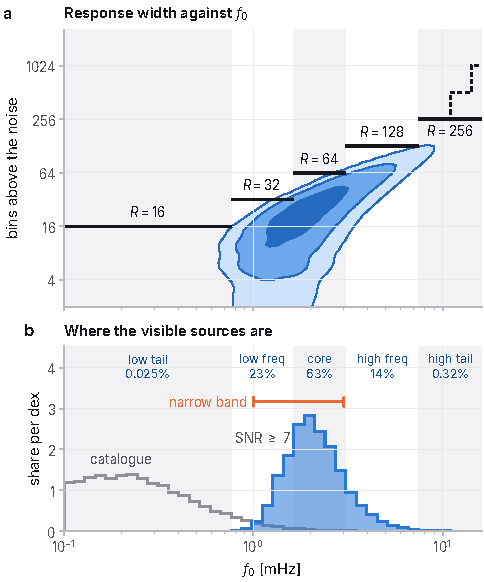
\includegraphics[width=\columnwidth]{figures/narrow-band.pdf}
  \caption{The band is divided where the response width doubles into five subbands (dotted
  vertical lines; \cref{tab:narrow-band-bands}). (a)~Response width: sources with power above the noise, by $f_0$ and by the
  bins that hold all of it; contours hold \qtylist{50;90;99}{\percent} of them. Solid segments: each subband's $R$, which keeps every above-noise bin of
  \qty{\NarrowBandSharePercent}{\percent} of the sources at each $f_0$; in the high tail that $R$
  (dashed) climbs to \NarrowBandTopR{}. (b)~Where the sources are: share per dex of $f_0$ of the catalogue's sources (grey)
  and of the visible ones, $\snr\ge\NarrowBandVisibleSnr$ (black), with each subband's share of the
  visible ones; the bracket marks the $f_0$ range of the narrow band.}
  \label{fig:narrow-band}
\end{figure}

\subsection{Visible Sources and Sources per Window}
\label{sec:gw-rates}\label{sec:narrow-band-prior}

\emph{Visible sources are rare and concentrated.} The catalogue puts
\qty{\NarrowBandLowTailCatalogue}{\percent} of its sources in the low tail, where they are faint;
the visible ones are its loud tail, and \qty{\NarrowBandCoreVisible}{\percent} of them fall in the
core (\cref{fig:narrow-band}b, \cref{fig:priors}a).

\emph{A window holds a known, small number of sources that matter.} Each of the
$N = \num{\RatesCatalogue}$ sources of the simulated Galaxy falls in a window with the probability
$p$ that the catalogue's marginal $\pi(f_0)$ puts there, so the window holds $n$ sources,
$n_{\rm vis}$ of them visible, with
\begin{equation}
\begin{gathered}
  n \sim \operatorname{Bin}\bigl(N, p\bigr),\qquad n_{\rm vis} \sim \operatorname{Bin}\bigl(N, p_{\rm vis}\bigr),\\
  p = \textstyle\int_{w} \pi(f_0)\,\dd f_0,\quad p_{\rm vis} = \textstyle\int_{w} \pi(f_0)\,P(\snr\ge\RatesVisibleSnr\mid f_0)\,\dd f_0.
\end{gathered}
  \label{eq:gw-rates}
\end{equation}
On average a window holds up to \num{\NarrowBandLowTailAllHi} sources at the bottom of the band,
almost none of them visible, and up to \num{\NarrowBandCoreVisibleHi} visible ones in its core
(\cref{tab:narrow-band-bands}, \cref{app:priors-counts}).

\subsection{Slots and the Trained Configurations}
\label{sec:narrow-band-bands}

Most sources of a window are below the noise, and for those the posterior is close to the prior. We
therefore fix the number of sources: every window holds exactly $S_w = S$ sources drawn from the
prior truncated to its interior, with $S$ set per run from 2 to 16, where a real analysis infers the
number with a trans-dimensional sampler \citep{littenberg2020global} and models the unresolved rest as
confusion noise \citep{karnesis2021characterization}. A slot the data do not resolve returns the
prior, and the flow works in a space of fixed dimension $8S$. A network of $S$ slots fits
\begin{equation}
  N_S = \int \frac{\dd f}{W(f)}\ \E\bigl[\min(n_{\rm vis},S)\mid f\bigr],\quad W = \ForwardModelWindowResponses{}R/\Tobs,
  \label{eq:narrow-band-fitted}
\end{equation}
visible sources over the divided band: \num{\NarrowBandFittedFour} at $S=4$,
\num{\NarrowBandFittedEight} at $S=8$ and \num{\NarrowBandFittedSixteen} at $S=16$, of
\num{\NarrowBandVisibleTotal} in the band, to be compared with the global fits of
\cref{tab:gw-globalfit}.

We train two configurations, each on one device. The \emph{narrow band},
\qtyrange{\PriorsNarrowLowMhz}{\PriorsNarrowHighMhz}{\milli\hertz} at $R=\ForwardModelNarrowR{}$, is
the core subproblem, holding \qty{\NarrowBandNarrowVisible}{\percent} of the visible sources where they
overlap most. The \emph{full band} covers the whole distribution at $R=\ForwardModelFullR{}$, the width
of the high-frequency subband: too narrow for the high tail, where
\qty{\NarrowBandHighTailVisible}{\percent} of the visible sources lose their outer bins
(\cref{sec:results-full}). Training all five subbands together is left to future work.
